% Section 8 -- Experiment 4: detection and task degradation on Llama-3.1-8B-Instruct.
% Included by paper.tex via \input{sections/experiment4}.
% Not a standalone file: it carries no preamble and no document environment.
% Graphics paths are relative to the manuscript root; in this repo the figures sit
% beside this file under docs/misc/figures/experiment4-llama/.
% Sources: results/experiment4/main (Slurm job 8333, 436,480 perturbed trials),
%          joined cell by cell against results/experiment1/full32_all.
% Figures: python code/analysis/plot_experiment4_layer_maps.py \
%              --run_dir results/experiment4/main --paper --format pdf \
%              --fields delta_accuracy --matchings alpha --no_error_bands \
%              --output_dir docs/misc/figures/experiment4-llama
%          then heatmap_alpha_delta_accuracy_light.pdf -> heatmap_alpha.pdf, etc.
%          depth_profile.pdf and surface_alpha.pdf are produced too and are unused here.

\section{Experiment 4: Detection Against Task Degradation}
\label{sec:exp4}

Experiment 1 establishes that a perturbation displaces the response logits toward the sentence it targets, and says nothing about what that perturbation costs the model.
If the displacement only appeared at doses where the computation is already destroyed, it would be compatible with disruption alone.
Experiment 4 instantiates the semantic classification control of \cref{sec:proposal} to bound that possibility.
The model is not questioned about the intervention here: it reads one labeled sentence under perturbation and answers whether that sentence expresses a queried concept, as a forced choice between two letters.

Three design constraints carry the experiment.
The queried concept is never the injected concept, which prevents a targeted injection from supplying the answer and, as a by-product, leaves the scored sentences disjoint from those that built the injected direction.
Both letter assignments are run on the same sentence, so that a preference for a letter is separable from a classification.
Blocks, families and both dose grids are those of Experiment 1, so every cell here pairs with a localization cell at the same block, family, matching and dose.

The sweep covers blocks 0--30, four families, ten raw amplitudes and twelve standardized doses over 80 items, for 436,480 perturbed trials and 80 sham trials.
The 80 items are five concepts from the complex-example corpus, four positive and four negative sentences each, under both mappings.
Cells are unequal by construction --- 80 trials for concept, 160 for renewed noise and for dropout, 240 for fixed random --- because the families carry two, two, two and three directions or realizations respectively; the sham baseline is the same 80 items throughout.
Block 31 is excluded because its concept directions cannot be rebuilt to the norm the calibration recorded, and by the argument of \cref{sec:exp1} it is structurally dead in any case.

Every measure derives from the logit difference between the two answer letters at the position that follows the assistant prefix,
\begin{equation}
 m = \operatorname{logit}(\text{correct letter}) - \operatorname{logit}(\text{other letter}),
 \label{eq:margin}
\end{equation}
whose exponential is the odds the model assigns the correct answer once the softmax is restricted to the two letters.
A trial scores 1 when $m>0$, 0 when $m<0$, and $0.5$ on an exact tie, so chance is 0.5 rather than 0.
Each perturbed trial carries the sham result of its own item, so accuracy change and margin change are matched item by item rather than pooled.

\subsection{The Control Task Is Performed, and the Reversed Mapping Is Required}

Without perturbation the model reaches 0.819 accuracy against the 0.5 forced-choice floor, at a 2.5\% invalid-answer rate and a mean margin of 2.86 logit, or odds near 17 to 1.
The control task is therefore informative rather than at floor, which is what makes a dose-dependent loss measurable.

The reversed mapping is not a formality.
The model answers X in 47 of the 80 sham trials, and that preference depresses exactly one cell of the design: positive sentences under the mapping in which Y means yes score 0.625, against 0.850 to 0.900 in the other three cells.
Pooling the mappings would have hidden a letter preference inside an apparent classification, exactly as the label-order counterbalancing of \cref{sec:exp1} exposes the A/B bias there.

\begin{figure*}[t]
\centering
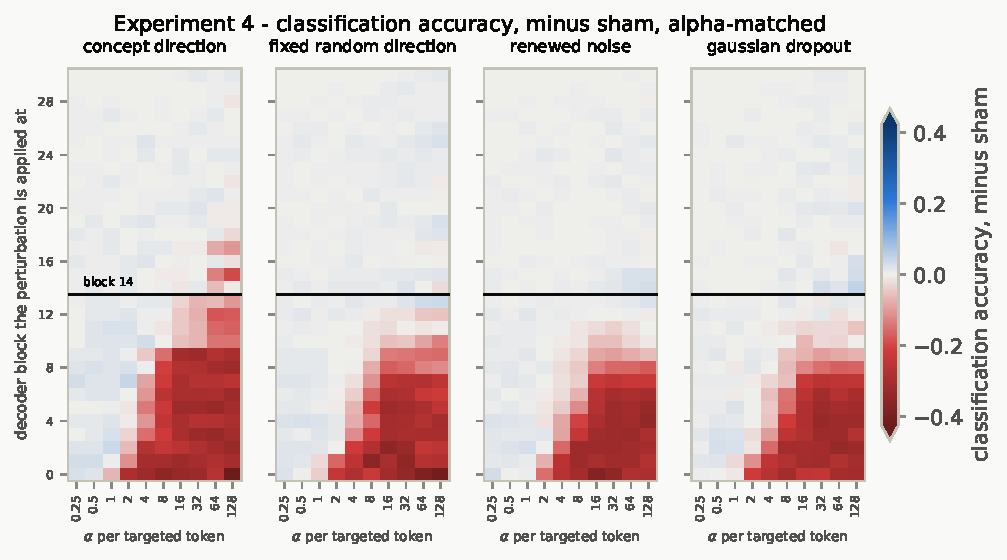
\includegraphics[width=0.97\textwidth]{figures/experiment4-llama/heatmap_alpha.pdf}
\caption{Classification accuracy minus sham by block and dose at matched raw amplitude, one panel per family. Red is degradation. The rule marks block 14, where the contiguous band of degraded blocks ends. The color scale is symmetric about zero by construction: fitted to the data it would stretch a $+6$ point sampling tail over half the ramp and render deep-block noise as vividly as shallow-block collapse.}
\label{fig:exp4heatmap}
\end{figure*}

\subsection{Degradation Ends at the Block Where Localization Ends}

\Cref{fig:exp4heatmap} shows the same qualitative structure in all four families: a degraded quadrant at low blocks and high doses, and a neutral region above it.
Pooling the four largest raw amplitudes, the contiguous band of blocks where some family loses at least 5 points of accuracy runs from block 0 and stops at block 14, and that boundary is stable for any threshold between 2 and 5 points.
This is the block at which localization also collapses in \cref{sec:exp1}, measured on a different task, a different prompt and a different corpus.
The two capacities --- disturbing the computation enough to break a semantic judgment, and displacing the logits toward the disturbed sentence --- end at the same depth.

The correspondence should not be over-read.
Beyond block 14 the concept family oscillates rather than staying flat: $-0.083$ at block 15, $0.000$ at block 16, $-0.050$ at block 17, $-0.003$ at block 18.
Isolated deep cells therefore survive the cut for that family, while Experiment 1 reports the deep localization zero as exact over 164,560 trials.
What is shared is the end of the contiguous band, not a claim that nothing happens above it.

\subsection{Concept Directions Disrupt Deeper Than Any Control}

At blocks 0--7 the four families are indistinguishable, all between $-0.23$ and $-0.36$: at high amplitude in the early stack, everything breaks the task equally.
From block 8 the controls recover and the concept family does not.

\begin{table}[H]
\centering
\small
\begin{tabular}{rrrrrr}
\toprule
Block & Concept & Fixed & Noise & Dropout & Gap \\
\midrule
7  & $-0.272$ & $-0.261$ & $-0.231$ & $-0.245$ & $-0.026$ \\
8  & $-0.295$ & $-0.144$ & $-0.157$ & $-0.152$ & $-0.144$ \\
9  & $-0.298$ & $-0.144$ & $-0.079$ & $-0.080$ & $-0.197$ \\
10 & $-0.103$ & $-0.081$ & $-0.038$ & $-0.031$ & $-0.053$ \\
12 & $-0.119$ & $-0.033$ & $0.000$  & $-0.004$ & $-0.106$ \\
15 & $-0.083$ & $0.014$  & $0.017$  & $0.014$  & $-0.098$ \\
18 & $-0.003$ & $0.010$  & $0.002$  & $0.003$  & $-0.008$ \\
\bottomrule
\end{tabular}
\caption{Classification accuracy minus sham, pooled over the four largest raw amplitudes. Fixed denotes fixed random directions. Gap is concept minus the mean of the three controls.}
\label{tab:exp4depth}
\end{table}

The deepest block at which the pooled loss still reaches 5 points is block 9 for renewed noise and for dropout, block 10 for fixed random directions, and block 15 for concept directions, with the gap peaking at $-0.197$ at block 9.
At matched raw amplitude a concept direction therefore disrupts this task five to six blocks further up the stack than any control.
This is a statement about disruption and not about reportability, and it inherits without modification the limitation of \cref{sec:exp1}: the concept vectors carry the attention-sink component, so a deeper reach is not yet attributable to conceptual content.

\begin{figure*}[t]
\centering
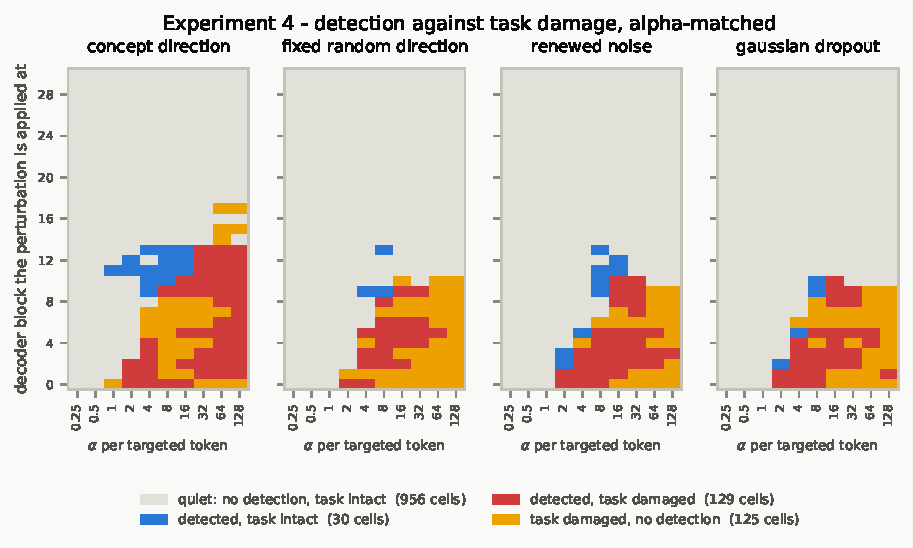
\includegraphics[width=0.97\textwidth]{figures/experiment4-llama/regimes_alpha.pdf}
\caption{Joint regimes at matched raw amplitude. A cell counts as detected when Experiment 1 localization accuracy reaches 70\%, and as damaged when classification accuracy falls more than 5 points below sham. Blue is the regime in which detection does not require disruption; in the concept panel those cells form a connected region at blocks 9--13.}
\label{fig:exp4regimes}
\end{figure*}

\subsection{Detection Without Disruption Exists, and Is Narrow}

Over all 2,728 paired cells, 682 per family, the two quantities move together.
Within each family, detectability and accuracy change correlate at $-0.724$ for concept, $-0.666$ for dropout, $-0.655$ for renewed noise and $-0.495$ for fixed random directions.
Accuracy change is negative when the task degrades, so these coefficients say that detection is generally higher where the disturbance is worse, which is what a disruption account predicts.

The exception is a minority of cells and it is not scattered.
Of the 1,240 cells matched on raw amplitude, 30 combine localization at 70\% or above with classification within 5 points of sham, and in the concept panel of \cref{fig:exp4regimes} they form a connected region spanning blocks 9--13 at amplitudes 1 through 16.
Connectedness in the block-by-dose plane is the argument: isolated cells are what chance produces, a connected region is not.
Over both dose rules 54 cells meet the criterion, 23 of them in the concept family.
Their Jensen--Shannon divergence from the sham output distribution has a median of 0.0019 bit, so the output distribution has barely moved where this holds.
Detection above chance can therefore coexist with success at this task, over a narrow band of the design; it does not follow that other capabilities are preserved there, nor that the mechanism is introspective.

\subsection{At Matched Degradation, Conceptual Content Buys Nothing}

Binning cells by accuracy loss and comparing detectability within each bin asks whether the concept family is distinguished by anything beyond the amount of damage it does.

\begin{table}[H]
\centering
\small
\begin{tabular}{lrrrr}
\toprule
Accuracy loss & Concept & Fixed & Noise & Dropout \\
\midrule
$[-1.00,-0.30)$ & 0.733 & 0.588 & 0.716 & 0.671 \\
$[-0.30,-0.15)$ & 0.712 & 0.659 & 0.688 & 0.693 \\
$[-0.15,-0.05)$ & 0.658 & 0.643 & 0.709 & 0.718 \\
$[-0.05,+0.05]$ & 0.521 & 0.508 & 0.518 & 0.516 \\
\bottomrule
\end{tabular}
\caption{Mean Experiment 1 localization accuracy at matched classification loss, both dose rules pooled. The comparison pools doses, so a family that reaches a bin at a much lower dose than another is not distinguished here.}
\label{tab:exp4matched}
\end{table}

Concept leads in the two heaviest bins, at 0.733 and 0.712, and falls behind in the third: 0.658 against 0.718 for dropout and 0.709 for renewed noise.
Subject to the pooling caveat, the comparison does not support the view that a conceptual perturbation is more reportable than a nonconceptual one of equal functional cost.
This is the same direction of result as the permuted-concept control of Experiment 1, obtained by an independent route.

\subsection{What the Sweep Does Not Establish}

\paragraph{The standardized results are not a family comparison.}
The $z$ grid was copied from the first Experiment 1 sweep so that cells would pair exactly, and that grid rests on the isolated-sentence calibration which \cref{sec:exp1} shows must not be interpreted.
The defect compounds here: the detection side of every standardized pairing is drawn from the same discredited sweep, and on the classification side the entire active region of all three controls is compressed into the four largest doses against the edge of the grid, so no control is ever tested near its own transition.
Nothing standardized in this section should be read as a difference between families.
The raw-amplitude results invoke no calibrated scale and are unaffected.
Repairing the standardized half requires rerunning this experiment against the behavioral-context calibration and the rebuilt grid of \cref{sec:exp1}.

\paragraph{The concept pairing is not matched across the join.}
The per-dose table of the localization sweep pools four concepts where this experiment injects two, so the concept row of every pairing relates neighboring but non-identical sets of directions.
The three control families are unaffected.

\paragraph{Output displacement, format compliance and task loss are three quantities.}
The invalid-answer rate rises from 2.5\% at sham to 94.2\% at its worst, and it fails independently of competence: at block 9 and amplitude 8 the concept family has already lost 15 points of accuracy while still emitting a valid letter on 97.5\% of trials.
Jensen--Shannon divergence separates from task loss just as sharply: at block 9 and amplitude 128, concept reaches 0.600 bit against 0.040 for renewed noise, a ratio of 15, while their accuracy losses are 29 and 6 points, a ratio of 5.
A large divergence is a changed output, not a failed task.

\paragraph{Dropout is matched only in expectation.}
Realized displacement tracks the request for the three additive families --- 128.04, 128.00 and 128.00 at block 9 for a request of 128 --- and undershoots for dropout at 112.70, whose amplitude is set through a rate rather than directly.
Dropout rows of the raw-amplitude comparison are therefore delivered slightly below their nominal dose.

\paragraph{Item counts.}
The 80 items rest on 5 concepts and 40 distinct sentences, each concept paired with a single injected direction.
Reported errors are trial-level, so between-item variability is not decomposed, and the concept-to-control comparisons in particular rest on two injected directions.

\paragraph{Summary.}
Detection and disruption are correlated across the design, which keeps a disruption account alive as the general case.
Against that, a connected region of the concept family at blocks 9--13 and moderate amplitude shows localization at 70\% or better while the control task holds within 5 points of sham and the output distribution barely moves, so detection does not require a broken computation everywhere.
At equal functional cost the conceptual perturbation is not more detectable than its controls, and the one place the concept family is clearly distinguished --- disrupting the task five to six blocks deeper --- is precisely the comparison that the sink component of the concept directions leaves unattributable.
The contiguous band of degraded blocks ends at block 14, where localization also ends.
